%\documentclass[12pt,preprint]{aastex}
\documentclass[iop]{emulateapj}
\usepackage{natbib,amsmath,graphicx,longtable,amssymb,latexsym,epsf}
\begin{document}

\title{Quasars Probing Quasars IX. Probing the Circumgalactic Flows of Quasars [v1.2]}

\author{Marie Wingyee Lau\altaffilmark{1}, J. Xavier Prochaska\altaffilmark{1}, 
Joseph F. Hennawi\altaffilmark{2}
}
\altaffiltext{1}{Department of Astronomy and Astrophysics, UCO/Lick Observatory, University of 
California, 1156 High Street, Santa Cruz, CA 95064}
\altaffiltext{2}{Max-Planck-Institut f\"ur Astronomie, K\"onigstuhl 17, D-69115 Heidelberg, 
Germany} 

\begin{abstract}
Absorption-line analysis of the circumgalactic medium has traditionally been limited by the 
difficulty to distinguish between inflows and outflows. We examine the flows of gas in the 
environments of massive galaxies hosting quasars at $z\sim2$. We employ 195 projected quasar pairs 
to study the circumgalactic gas of the foreground quasars in absorption. The foreground quasars 
have precise redshift measurements with uncertainty $<400\,{\rm km\,s^{-1}}$. We stack the 
background quasar spectra at the foreground quasar's systemic redshift. The mean absorption in 
\ion{C}{2}, \ion{C}{4}, and \ion{Mg}{2} show large intrinsic velocity fields, and have velocity 
centroids that show a small positive offset relative to the systemic. We argue the results can be 
explained by outflowing gas combined with anisotropic or intermittent ionizing radiation of the 
quasars. 
\end{abstract}


\keywords{glaxies: clusters: intracluster medium -- galaxies: formation -- galaxies: halos -- 
intergalactic medium -- quasars: absorption lines -- quasars: general}

\section{Introduction}
\label{sec:introduction}
%\begin{itemize}
%\item Flows
%\item Mass (Kaiser, Schaye)
%\item Directionality/symmetry
%\item Break the symmetry
%\end{itemize}

Galaxy formation and evolution are driven by the flows into and out of their interstellar medium. 
Current theories demand that star-forming galaxies maintain these flows. Gas accretes, cools, and 
adds to the fuel supply, while star formation feedback heats gas, blows it out of galaxies, and 
regulates star formation \citep[for a review see][]{SomervilleDave15}. 

Direction observations of galactic flows are difficult to acquire. Detecting the presence of 
the gas is itself challenging. Either the gas mass is too small, or the gas density is too low for 
the detection of line-emission, e.g.\ 21\,cm, Ly$\alpha$, or H$\alpha$ from \ion{H}{1}. Resolving 
the kinematics and establishing the mass flux pose an even greater challenge. These challenges are 
accentuated for distant, young galaxies, where flows are predicted to prevail 
\citep{Keres+09,Fumagalli+11}. Therefore, with rare exceptions, 
\citep[e.g.][]{Cantalupo+14,Hennawi+15}, the community has relied on absorption-line spectroscopy 
to detect and characterize the gas surrounding galaxies 
\citep[e.g.][]{BergeronBoisse91,Steidel+10,Prochaska+11,Tumlinson+13}. With this 
experiment, researchers have had success in characterizing the large-scale flows around 
star-forming galaxies to reveal a net inflow, or a Kaiser effect for gas \citep{Rakic+12}. 

A significant limitation of absorption-line analysis, especially regarding galactic flows, 
is the inherent symmetry of the experiment. One generally lacks any constraint on the distance of 
the gas along the sightline. Positive or negative velocities with respect to the galaxy may be 
interpreted as gas flowing either toward or away from the system. ``Down-the-barrel'' observations 
break this symmetry, and have generally provided evidence for flows away from galaxies 
\citep{Rupke+05,Martin05,Weiner+09,Rubin+14}. However, these data are frequently at low spectral 
resolution which limits one's sensitivity to inflowing gas. 

In this paper (hereafter QPQ9), we examine the flows of gas in the environments of massive 
galaxies hosting quasars. Our approach leverages a large dataset of quasar pairs 
\citep[][QPQ1]{QPQ1} to use the 
standard technique of absorption-line spectroscopy with background quasars. These quasar pairs 
have angular separations that correspond to less than 300\,kpc projected separation at the 
foreground quasar's redshift. Our previous publications from these quasar pairs have established 
that these galaxies are surrounded by a massive, cool, and enriched circumgalactic medium 
\citep[QPQ5, QPQ6, QPQ7:][]{QPQ5,QPQ6,QPQ7}. We have collected a sample of 195 background 
spectra that are paired with foreground quasars with precisely measured redshifts. Our primary 
scientific interests are twofold: (i) search for signatures of galactic-scale outflows from the 
central galaxy, presumably driven by recent star formation and/or active galactic nuclei feedback; 
(ii) characterize the dynamics of galactic flows around these massive system. We further describe 
an aspect of this experiment that offers a unique opportunity to study galactic flows: we argue 
that, the anisotropic or intermittent radiation of the foreground quasars breaks the symmetry in 
the velocity field of circumgalactic absorbers. 

Among the sightlines in the QPQ9 sample, 13 have spectral resolution $> 5000$ from echellette or 
echelle observations, and have been analyzed separately in QPQ8 \citep{QPQ8}. We measured the 
velocity field for \ion{C}{2}\,1334 and \ion{C}{4}\,1548, finding that the CGM frequently exhibits 
large flows that are offset from the systemic redshift. The offsets, $\delta v$, are often 
positive, with the sign convention that positive velocities are flowing away from the observer. 
From a sample of 7 \ion{C}{2} systems and 10 \ion{C}{4} systems, we measured the velocity 
interval that encompasses 90\% of the total optical depth, $\Delta v_{90}$, and the $1\sigma$ 
dispersion relative to the profile centroid, $\sigma_v$. The median $\Delta v_{90}$ is 
$555\,{\rm km\,s^{-1}}$ for \ion{C}{2}\,1334 and is $342\,{\rm km\,s^{-1}}$ for \ion{C}{4}\,1548. 
The median $\sigma_v$ is $249\,{\rm km\,s^{-1}}$ for \ion{C}{2}\,1334 and is 
$495\,{\rm km\,s^{-1}}$ for \ion{C}{4}\,1548. These velocity fields exceed all previous 
measurements from galaxies and/or absorption systems at any epoch. 

%The formation and evolution of stars are dictated
%by the flow of gas and metals/dust.  [This transport
%varies directly with the stellar stage
%and a lesser extent stellar mass.]
%The accretion onto a protostellar  core eventually
%initiates nuclear fusion.  The main sequence is characterized
%by gentler stellar winds, with the most massive
%stars shedding a cumulative mass of XX\%.
%Stellar deaths, meanwhile, are frequently accompanied by terrific
%mass loss, occasionally punctuated by a highly energetic,
%supernova phase.
%By analogy, galaxy formation and evolution are driven by the
%flows into/out of their interstellar medium.
%In contrast to most stars, however, current theories
%predict (even demand) that the star-forming galaxies
%maintin these flows. [add]
%Akin to stars, direct observations of galactic flows are
%difficult to acquire. Even detecting the gas is challenging:
%the gas mass is either too small or the gas density too low
%for the [detection] of line-emission (e.g. 21cm, lya,
%or H$\alpha$ from Hydrogen).  Resolving the kinematics
%and establish the mass-flux represent a far greater challenge.
%These challenges are accentuated for distant, young galaxies
%where flows are predicted to prevail \citep{keres,fumagalli}.
%Therefore, with rare exceptions \citep[e.g.][]{slug,jackpot},
%the community has relied on absorption-line spectroscopy
%to detect and characterize the gas surrounding galaxies
%\citep[e.g.][]{bergeron,steidel10,pro11,tumlinson13}.
%With this experiment, researcher have had recent success
%in characterizing the large-scale flows around star-forming
%galaxies to reveal a net inflow \cite{rakic13} and
%provide unique constraints on the mass of the underlying
%potential well \cite{rakic14}.
%A significant limitation of standard absorption-line
%analysis, especially regarding sutyding galactic flows,
%is the inherent symmetry of the experiment.
%Because one generally lacks any constraint on the distance
%of the gas along the sightline,
%postive or negative velocities with respect to the
%galaxy may be interpreted as gas flowing either towards
%or away from the system.
%So-called `down-the-barrel' observations break this
%symmetry, and have generally provided evidence for flows
%away from galaxies \citep{rupke,martin,weiner,rubin}.
%However, these data are frequently at low spectral resolution
%which limits one's sensitivity to inflowing gas.
%In this paper, we examine the flows of gas in the environments
%of massive galaxies hosting quasars.  Our approach leverages
%a large dataset of quasar pairs \citep{hennawi}
%to use the standard technique of absorption-line spectroscopy
%with background quasars. [word]
%These quasar pairs have angular
%separations that correspond to less than 300\,kpc physical
%separation at the f/g quasar redshift.
%Our previous publications from these quasar pairs
%have established that these galaxies are surrounded
%by a massive, cool, and enriched circumgalactic medium
%\citep{QPQ1,QPQ5,QPQ6,QPQ7}.
%We have collected a sample of ntot~spectra passing within
%300\,kpc from a f/g quasar with a precisely measured
%redshift.  Our primary scientific interests are twofold:
%(i) search for signatures of galactic-scale outflows from the
%central galaxy, presumably driven by recent star-formation
%and/or AGN feedback;
%(ii) characterize the dynamics of galactic flows around these
%massive system.  We further descrbie an aspect of this
%experiment that offers a unique opportunity to study galactic
%flows. [detail??]

We adopt a $\Lambda$CDM cosmology with $\Omega_M=0.26, \Omega_\Lambda=0.74$, and 
$H_0=70\,{\rm km\,s^{-1}\,Mpc^{-1}}$. Distances are proper unless otherwise stated. When referring 
to comoving distances we include explicitly an $h^{-1}$ term and follow modern convention of 
scaling to a Hubble constant of $70\,{\rm km\,s^{-1}\,Mpc^{-1}}$. 
%All equivalent width measurements are presented in the rest-frame, unless otherwise specified. 

\section{The Experiment}
\label{sec:experiment}

\begin{figure}
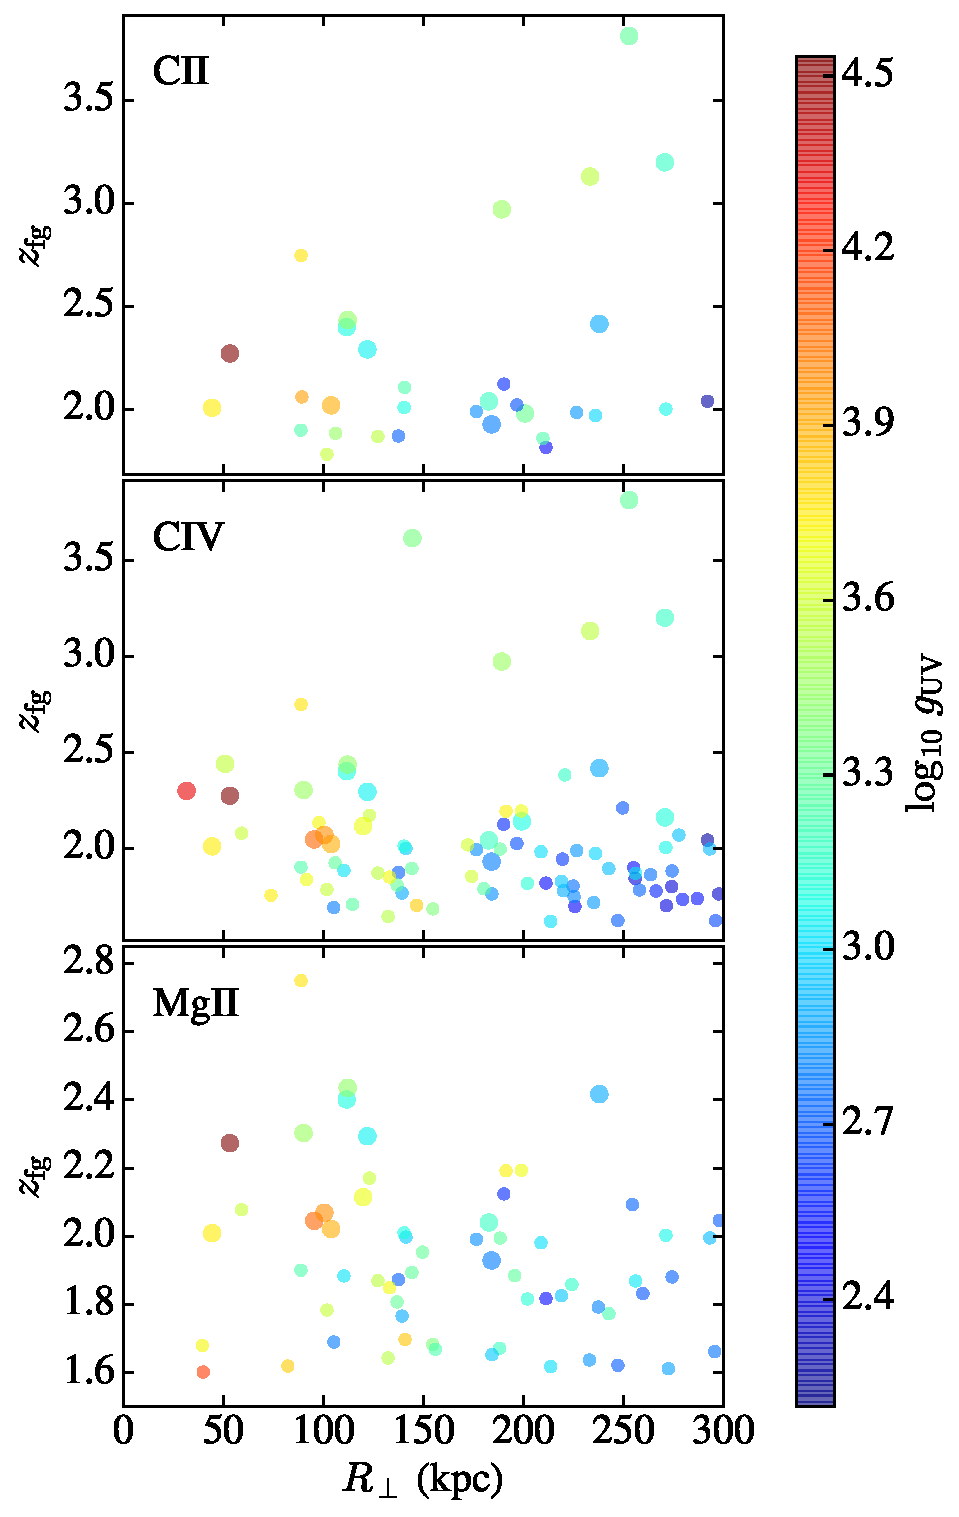
\includegraphics[width=3in]{Figures/fig_experiment.pdf}
\caption{These panels summarize properties of the QPQ9 dataset. The QPQ survey selects 
quasar pairs of $R_\perp < 300$\,kpc and $z_{\rm fg}>1.6$. Assuming that the foreground quasars 
emit isotropically and at a distance equal to the impact parameter, the aenhancement in the UV 
flux relative to the extragalactic UV background, $g_{\rm UV}$, can be estimated. Large 
symbols correspond to foreground quasars with the most precise redshift measurement from 
[\ion{O}{3}]\,5007, while small symbols correspond to $z_{\rm fg}$ 
measurements from \ion{Mg}{2}\,2800, H$\alpha$, or H$\beta$ emission. The top panel shows 
quasar pairs with coverage of \ion{C}{2}\,1334 at $z_{\rm fg}$ in the background quasar spectra. 
The middle panel shows pairs with coverage of \ion{C}{4}\,1548. The bottom panel shows 
pairs with coverage of \ion{Mg}{2}\,2796. 
}
\label{fig:experiment}
\end{figure}

The goal of our experiment is to measure the average velocity fields of the absorption from C$^+$, 
C$^{3+}$, and Mg$^+$ ions associated with the CGM of the massive galaxies hosting $z\sim 2$ 
quasars. 

From our QPQ survey\footnote{http://www.qpqsurvey.org}, we have analyzed a subset of systems that 
pass within transverse separation $R_\perp<300$\,kpc from a foreground quasar with 
$z_{\rm fg} > 1.6$. We restrict the sample to foreground quasars with redshift measured from 
\ion{Mg}{2}\,2800, [\ion{O}{3}]\,5007, H$\alpha$, or H$\beta$ emission, giving a precision of 
$400\,{\rm km\,s^{-1}}$ or better. 
[\ion{O}{3}] emission-line redshifts have the smallest dispersion of $44\,{\rm km\,s^{-1}}$ about 
the systemic redshift, and we analyze the sub-sample with [\ion{O}{3}] redshifts separately. 
The [\ion{O}{3}] line has an average blueshift of $27\,{\rm km\,s^{-1}}$ about the systemic 
redshift \citep{Boroson05}, which has been added when we compute the 
redshift of the line. Systemic redshifts measured from \ion{Mg}{2} have a precision of 
$272\,{\rm km\,s^{-1}}$, and we have taken into account the median redshift of 
$97\,{\rm km\,s^{-1}}$ of \ion{Mg}{2} from [\ion{O}{3}] \citep{Richards+02}. In QPQ8 
\citep{QPQ8}, we have quantified the precision of H$\alpha$ and H$\beta$ to be 
$300\,{\rm km\,s^{-1}}$ and $392\,{\rm km\,s^{-1}}$ respectively. We further add to the QPQ 
dataset with quasar pairs selected from the public dataset of 
igmspec\footnote{https://github.com/specdb/igmspec}, which includes the spectra from the quasar 
catalogs based upon the Sloan Digital Sky Survey Seventh Data Release \citep{Schneider+10} and the 
Twelfth Data Release \citep{Paris+17}. We 
only select pairs with $z_{\rm fg}$ measured by \cite{HewettWild10} using the \ion{Mg}{2}\,1800 
emission-line. We reached a final sample size of 195. Figure~\ref{fig:experiment} summarizes the 
experimental design. We refer the reader to previous QPQ publications for the details on the 
redshift centroiding algorithm, data reduction, and continuum normalization (QPQ6; QPQ8). 

As in the previous QPQ papers, we select the quasar pairs to have redshift difference 
$>3000\,{\rm km\,s^{-1}}$, to exclude physically associated binary quasars. The cut on velocity 
difference is motivated by the typical redshift uncertainty of $\approx500\,{\rm km\,s^{-1}}$ of 
the background quasars. In QPQ8, it was required that the observed wavelengths of the 
metal ion transitions fall outside the Ly$\alpha$ forest of the background quasar. In this paper, 
we exclude a small window around the Ly$\alpha$ emission, in additional to the Ly$\alpha$ forest, 
from analysis. For stacked profile analysis, a good estimate of 
the continuum level is neessary. In QPQ8 we found that absorption associated to 
the foreground quasar occurs within $\pm2000\,{\rm km\,s^{-1}}$ around $z_{\rm fg}$. Therefore, it 
is desirable to keep a $\approx\pm3000\,{\rm km\,s^{-1}}$ window relatively free of contamination 
from Ly$\alpha$ forest. Taking into account the redshift uncertainties, 
we decide that at least one transition among \ion{C}{2}\,1334, \ion{C}{4}\,1548, and 
\ion{Mg}{2}\,2796 at $z_{\rm fg}$ must lie redward of 
$(1215.6701+20)\times(1+z_{\rm bg})\,{\rm \AA}$, for a pair to be included in the analysis. 

Furthermore, we include only those spectra with average signal-to-noise ratio (S/N) exceeding 5.5 
per rest-frame \AA \ in a $\pm3000\,{\rm km\,s^{-1}}$ window centered on the observed wavelengths 
of the metal ion transitions. This criterion is a compromise between maximizing sample size versus 
maintaining good data quality on the individual sightlines. We find that S/N $>5.5$ per rest-frame 
\AA \ is 
necessary for properly estimating the continuum, as well as identifying mini-broad absorption line 
systems associated to the background quasar, which will significantly depress the flux level. We 
also require that the region of the spectrum that is $\pm3000\,{\rm km\,s^{-1}}$ around a 
considered metal ion transition does not overlap with strong atmospheric ${\rm O}_2$ bands. 
The ${\rm O}_2$ A- and B-band span 7595\textendash7680\,\AA \ and 6868\textendash6926\,\AA \ 
respectively. 

Table~\ref{tab:sample} lists the full QPQ9 sample. 
In Table~\ref{tab:summary}, we list the sample size, the median $z_{\rm fg}$, and the median 
$R_\perp$ of the quasar pairs that survive the above selection criteria for \ion{C}{2}\,1334, 
\ion{C}{4}\,1548, and \ion{Mg}{2}\,2796 respectively. In Table~\ref{tab:summary_OIII}, we provide 
the summary for the sub-sample with $z_{\rm fg}$ measured from [\ion{O}{3}]. 

\LongTables
\begin{deluxetable*}{ccccccccc}
\tablewidth{0pc}
\tablecaption{Properties of the Projected Quasar Pairs in the QPQ9 sample\label{tab:sample}}
\tabletypesize{\scriptsize}
\setlength{\tabcolsep}{0in}
\tablehead{\colhead{Foreground Quasar} & \colhead{$z_{\rm fg}$} & 
\colhead{Line for $z_{\rm fg}^a$} & \colhead{Background Quasar} & 
\colhead{$z_{\rm bg}$} & \colhead{BG Quasar Instrument} & 
\colhead{$R_\perp$ (kpc)} & \colhead{$g_{\rm UV}$}} 
\startdata 
J004757.26+144741.0 & 1.6191 & MgII & J004757.88+144744.7 & 2.757 & BOSS & 82 & 6705 \\ 
J005717.36$-$000113.3 & 2.1611 & [OIII] & J005718.99-000134.7 & 2.511 & BOSS & 271 & 1283 \\ 
J010323.84$-$000254.2 & 1.7506 & MgII & J010324.37-000251.3 & 2.306 & BOSS & 74 & 5488 \\ 
J014917.11$-$002141.6 & 1.6834 & MgII & J014917.46-002158.5 & 2.159 & SDSS & 155 & 2390 \\ 
J021416.96$-$005229.1 & 1.8002 & MgII & J021416.12-005251.5 & 2.332 & BOSS & 225 & 566 \\ 
J022447.89$-$004700.4 & 1.6959 & MgII & J022448.85-004638.9 & 2.188 & BOSS & 226 & 294 \\ 
J023018.27$-$033319.4 & 2.3817 & MgII & J023019.99-033315.0 & 2.985 & BOSS & 221 & 1444 \\ 
J023946.43$-$010640.4 & 2.299 & [OIII] & J023946.45-010644.1 & 3.124 & BOSS & 32 & 20931 \\ 
J025038.69$-$004739.1 & 1.8538 & MgII & J025039.82-004749.6 & 2.444 & BOSS & 174 & 4033 \\ 
J034138.16+000002.9 & 2.1246 & MgII & J034139.19-000012.7 & 2.243 & GMOS-N & 190 & 392 \\ 
J040955.87$-$041126.9 & 1.7166 & MgII & J040954.21-041137.1 & 2.0 & MagE & 235 & 715 \\ 
J075259.81+401128.2 & 1.8844 & MgII & J075259.14+401118.2 & 2.121 & SDSS & 110 & 1060 \\ 
J080049.89+354249.6 & 1.9825 & [OIII] & J080048.74+354231.3 & 2.066 & LRIS & 201 & 2074 \\ 
J080945.17+453918.1 & 2.0392 & MgII & J080948.22+453929.0 & 2.278 & BOSS & 292 & 195 \\ 
J081223.17+262000.9 & 1.6427 & MgII & J081223.89+262012.5 & 2.17 & BOSS & 132 & 3446 \\ 
J081419.58+325018.7 & 2.1744 & [OIII] & J081420.38+325016.1 & 2.213 & GMOS-N & 90 & 0 \\ 
J081832.87+123219.9 & 1.7032 & MgII & J081833.97+123215.4 & 2.234 & BOSS & 147 & 6606 \\ 
J082642.86+470829.5 & 1.8085 & MgII & J082644.64+470803.9 & 1.861 & SDSS & 274 & 250 \\ 
J082843.37+454517.3 & 1.873 & MgII & J082844.87+454518.2 & 1.987 & LRIS & 137 & 525 \\ 
J083030.38+545228.8 & 1.6702 & MgII & J083029.11+545210.3 & 3.337 & BOSS & 188 & 1509 \\ 
J083713.56+363037.3 & 1.8364 & MgII & J083712.69+363037.7 & 2.301 & MODS1 & 92 & 5012 \\ 
J083757.91+383727.1 & 2.0624 & H$\alpha$ & J083757.13+383722.4 & 2.251 & LRIS & 89 & 8609 \\ 
J083854.52+462124.4 & 1.7596 & MgII & J083852.94+462137.6 & 2.163 & BOSS & 184 & 675 \\ 
J084158.47+392120.0 & 2.0414 & [OIII] & J084159.26+392139.0 & 2.214 & LRIS & 183 & 1514 \\ 
J085358.36$-$001108.0 & 2.4016 & [OIII] & J085357.49-001106.2 & 2.579 & MagE & 112 & 1231 \\ 
J085629.48+551450.2 & 1.6228 & MgII & J085630.45+551417.5 & 1.932 & BOSS & 296 & 466 \\ 
J085737.58+390120.5 & 1.9529 & MgII & J085738.00+390136.0 & 2.848 & BOSS & 150 & 1987 \\ 
J090417.94+004148.2 & 1.6193 & MgII & J090419.12+004205.1 & 1.645 & SDSS & 214 & 1034 \\ 
J090657.78+100121.4 & 1.6965 & MgII & J090657.62+100105.6 & 2.525 & BOSS & 141 & 6972 \\ 
J091046.44+041458.5 & 2.0461 & [OIII] & J091046.69+041448.4 & 2.377 & MagE & 95 & 11897 \\ 
J091217.57+413933.5 & 1.7764 & MgII & J091215.75+413948.2 & 2.198 & BOSS & 220 & 792 \\ 
J091234.27+305616.2 & 1.6237 & MgII & J091236.32+305626.5 & 2.146 & BOSS & 247 & 514 \\ 
J091338.33$-$010708.7 & 2.7491 & MgII & J091338.97-010704.6 & 2.916 & XSHOOTER & 89 & 5830 \\ 
J091432.02+010912.4 & 2.1404 & [OIII] & J091430.85+010927.5 & 2.475 & BOSS & 199 & 1222 \\ 
J091551.72+011900.2 & 1.9706 & MgII & J091553.37+011911.4 & 2.102 & BOSS & 236 & 972 \\ 
J092417.65+392920.3 & 1.8864 & MgII & J092416.72+392914.6 & 2.08 & LRIS & 106 & 2788 \\ 
J093226.34+092526.1 & 2.4172 & [OIII] & J093225.66+092500.2 & 2.602 & MagE & 238 & 774 \\ 
J093317.43+592027.4 & 1.8617 & MgII & J093320.57+592036.5 & 2.633 & BOSS & 224 & 1437 \\ 
J093640.35$-$005840.1 & 2.2098 & MgII & J093642.12-005831.3 & 2.731 & BOSS & 250 & 496 \\ 
J094133.64+230840.1 & 1.7762 & MgII & J094135.61+230845.8 & 2.551 & BOSS & 243 & 1696 \\ 
J100046.45+033708.8 & 1.7006 & MgII & J100048.52+033708.8 & 2.353 & BOSS & 271 & 255 \\ 
J100509.56+501929.8 & 1.8176 & MgII & J100507.07+501929.8 & 2.019 & LRIS & 211 & 330 \\ 
J100627.47+480420.0 & 2.3034 & [OIII] & J100627.11+480429.9 & 2.597 & BOSS & 90 & 2886 \\ 
J100913.91+023612.4 & 1.7359 & MgII & J100913.33+023643.0 & 2.216 & BOSS & 287 & 342 \\ 
J100941.35+250104.1 & 1.8703 & MgII & J100940.58+250053.9 & 1.981 & LRIS & 127 & 3588 \\ 
J101001.51+403755.5 & 2.1924 & H$\alpha$ & J101003.47+403754.9 & 2.505 & BOSS & 191 & 5421 \\ 
J101323.89+033016.0 & 1.9401 & MgII & J101322.23+033009.1 & 2.273 & BOSS & 219 & 428 \\ 
J101753.38+622653.4 & 1.6528 & MgII & J101750.44+622648.2 & 2.738 & BOSS & 184 & 923 \\ 
J102007.23+611955.0 & 1.7909 & MgII & J102010.05+611950.3 & 2.387 & BOSS & 180 & 1813 \\ 
J103443.62+085702.0 & 1.6395 & MgII & J103442.26+085645.7 & 2.766 & BOSS & 233 & 699 \\ 
J103628.12+501157.9 & 2.0097 & MgII & J103630.52+501219.8 & 2.228 & BOSS & 271 & 1191 \\ 
J103857.37+502707.0 & 3.1325 & [OIII] & J103900.01+502652.8 & 3.236 & ESI & 233 & 3567 \\ 
J104244.84+650002.7 & 1.9876 & MgII & J104245.14+645936.7 & 2.124 & BOSS & 227 & 703 \\ 
J104435.62+313950.7 & 1.7062 & MgII & J104434.76+313957.7 & 2.377 & BOSS & 115 & 1875 \\ 
J105221.77+555253.5 & 1.9989 & MgII & J105218.36+555311.3 & 2.278 & BOSS & 293 & 844 \\ 
J111339.86+330604.8 & 1.8913 & MgII & J111337.84+330553.3 & 2.413 & BOSS & 243 & 855 \\ 
J111850.44+402553.8 & 1.9257 & MgII & J111851.45+402557.6 & 2.317 & BOSS & 106 & 1944 \\ 
J113852.65+632934.0 & 1.8855 & MgII & J113851.73+632955.6 & 2.625 & BOSS & 196 & 1912 \\ 
J114435.54+095921.7 & 2.9734 & [OIII] & J114436.65+095904.9 & 3.16 & MIKE-Red & 189 & 2914 \\ 
J114546.54+032236.7 & 1.7664 & MgII & J114546.22+032251.9 & 2.011 & MagE & 139 & 779 \\ 
J115253.09+150706.5 & 1.7883 & MgII & J115254.97+150707.8 & 3.349 & BOSS & 237 & 626 \\ 
J115533.62+393359.2 & 1.6118 & MgII & J115531.32+393415.4 & 2.555 & BOSS & 272 & 742 \\ 
J120224.68+074800.3 & 1.6613 & MgII & J120226.48+074739.7 & 2.767 & BOSS & 296 & 584 \\ 
J120417.47+022104.7 & 2.436 & [OIII] & J120416.69+022110.0 & 2.532 & HIRES & 112 & 2710 \\ 
J120856.94+073741.2 & 2.1708 & MgII & J120857.16+073727.3 & 2.616 & MagE & 123 & 3853 \\ 
J121159.88+324009.0 & 1.978 & MgII & J121201.69+324013.3 & 2.273 & BOSS & 209 & 1050 \\ 
J121344.28+471958.7 & 1.8371 & MgII & J121343.01+471931.0 & 3.275 & BOSS & 260 & 488 \\ 
J1215590+571616.6 & 1.93 & [OIII] & J121558.82+571555.5 & 1.964 & SDSS & 184 & 614 \\ 
J122514.29+570942.3 & 1.8953 & MgII & J122517.89+570943.7 & 2.224 & BOSS & 255 & 331 \\ 
J123143.01+002846.3 & 3.2015 & [OIII] & J123141.73+002913.9 & 3.308 & GMOS-S & 271 & 1490 \\ 
J124632.33+234531.2 & 1.9937 & MgII & J124632.19+234509.5 & 2.573 & BOSS & 188 & 1889 \\ 
J124846.05+405758.2 & 1.8265 & MgII & J124846.97+405820.9 & 2.463 & BOSS & 219 & 897 \\ 
J130124.74+475909.6 & 2.194 & H$\alpha$ & J130125.67+475930.8 & 2.765 & SDSS & 199 & 4932 \\ 
J130605.19+615823.7 & 2.1089 & H$\alpha$ & J130603.55+615835.2 & 2.175 & LRIS & 141 & 1761 \\ 
J132514.97+540930.6 & 2.0507 & MgII & J132511.07+540927.0 & 3.235 & BOSS & 298 & 513 \\ 
J134650.08+195235.2 & 2.0697 & MgII & J134648.19+195253.1 & 2.523 & BOSS & 278 & 883 \\ 
J135849.71+273806.9 & 1.9008 & MgII & J135849.54+273756.9 & 2.127 & LRIS & 89 & 1765 \\ 
J141337.18+271517.1 & 1.6905 & MgII & J141337.96+271511.0 & 1.965 & BOSS & 105 & 609 \\ 
J142003.67+022726.7 & 3.617 & [OIII] & J142004.12+022708.8 & 4.191 & ESI & 144 & 2291 \\ 
J142054.42+160333.3 & 2.0221 & [OIII] & J142054.92+160342.9 & 2.057 & MagE & 104 & 7811 \\ 
J142215.57+465230.7 & 1.748 & MgII & J142214.63+465254.6 & 2.338 & BOSS & 225 & 639 \\ 
J142758.89$-$012130.4 & 2.2738 & [OIII] & J142758.74-012136.2 & 2.354 & MIKE & 53 & 34208 \\ 
J143109.67+572728.0 & 1.6802 & MgII & J143109.22+572726.4 & 2.063 & BOSS & 39 & 5166 \\ 
J143312.56+082651.8 & 1.8807 & MgII & J143313.99+082714.0 & 2.432 & BOSS & 274 & 531 \\ 
J143345.55+064109.0 & 2.294 & [OIII] & J143344.55+064111.9 & 2.34 & BOSS & 122 & 1130 \\ 
J144232.92+013730.4 & 1.8079 & MgII & J144231.91+013734.8 & 2.274 & BOSS & 137 & 1988 \\ 
J150814.06+363529.4 & 1.8493 & MgII & J150812.78+363530.3 & 2.105 & BOSS & 133 & 5111 \\ 
J153328.83+142542.5 & 2.0782 & MgII & J153329.17+142537.8 & 2.564 & BOSS & 59 & 3898 \\ 
J153456.02+215342.3 & 1.6712 & MgII & J153455.85+215324.7 & 2.529 & BOSS & 156 & 1700 \\ 
J153954.74+314629.3 & 1.8747 & MgII & J153952.46+314625.2 & 2.235 & BOSS & 256 & 1075 \\ 
J155325.61+192140.0 & 2.01 & [OIII] & J155325.89+192137.7 & 2.098 & MagE & 44 & 5576 \\ 
J155422.88+124438.0 & 1.8169 & MgII & J155424.39+124431.5 & 2.394 & BOSS & 202 & 1350 \\ 
J155947.73+494307.3 & 1.8615 & MgII & J155946.28+494326.7 & 1.945 & LRIS & 210 & 1743 \\ 
J160547.59+511330.2 & 1.783 & MgII & J160546.66+511322.6 & 1.849 & LRIS & 102 & 3813 \\ 
J161930.94+192620.9 & 1.7821 & MgII & J161929.78+192645.4 & 2.39 & BOSS & 258 & 538 \\ 
J162738.63+460538.4 & 3.8149 & [OIII] & J162737.25+460609.3 & 4.11 & ESI & 253 & 1959 \\ 
J163121.74+433317.3 & 2.0182 & MgII & J163123.57+433317.3 & 2.631 & BOSS & 172 & 4088 \\ 
J165716.85+310513.0 & 2.1331 & MgII & J165716.52+310524.5 & 2.395 & MODS1 & 98 & 5222 \\ 
J214620.69$-$075250.6 & 2.1155 & [OIII] & J214620.99-075303.8 & 2.577 & MagE & 120 & 4869 \\ 
J220248.61+123645.5 & 2.0697 & [OIII] & J220248.31+123656.3 & 2.512 & BOSS & 100 & 9466 \\ 
J225535.67$-$000156.8 & 1.7302 & MgII & J225537.62-000144.1 & 2.412 & BOSS & 280 & 352 \\ 
J233845.19$-$000327.1 & 2.4399 & [OIII] & J233845.45-000331.8 & 2.997 & XSHOOTER & 51 & 3745 \\ 
\enddata 
\tablenotetext{a}{The emission-line analyzed for measuring $z_{\rm fg}$.} 
\end{deluxetable*}
\begin{deluxetable*}{lccc}
\tablewidth{0pc}
\tablecaption{Summary of Experimental Design and Analysis for the Full QPQ9 Sample
\label{tab:summary}}
\tabletypesize{\small}
\tablehead{\colhead{Measure} & \colhead{\ion{C}{2}\,1334} & \colhead{\ion{C}{4}\,1548} 
& \colhead{\ion{Mg}{2}\,2796}} 
\startdata 
Number of pairs & 34 & 92 & 26 \\ 
Median $z_{\rm fg}$ & 2.03 & 1.94 & 1.88 \\ 
Median $R_\perp$ (kpc) & 180 & 189 & 150 \\ 
Centroid of mean-stacked spectrum (${\rm km\,s^{-1}}$) & $+170\pm121$ & $+53\pm105$ & $+161\pm108$ \\
1$\sigma$ dispersion of mean stack (${\rm km\,s^{-1}}$) & 388 & 363 & 340 \\
Centroid of median-stacked spectrum (${\rm km\,s^{-1}}$) & $+16\pm106$ & $+181\pm106$ & $-12\pm162$ \\
1$\sigma$ dispersion of median stack (${\rm km\,s^{-1}}$) & 313 & 320 & 207 \\
\enddata 
\end{deluxetable*} 

\begin{deluxetable*}{lccc}
\tablewidth{0pc}
\tablecaption{Summary for the Sub-sample with $z_{\rm fg}$ Measured from [\ion{O}{3}] 
\label{tab:summary_OIII}}
\tabletypesize{\scriptsize}
\setlength{\tabcolsep}{0in}
\tablehead{\colhead{Measure} & \colhead{\ion{C}{2}\,1334} & \colhead{\ion{C}{4}\,1548} 
& \colhead{\ion{Mg}{2}\,2796}} 
\startdata 
Number of pairs & 14 & 22 & 9 \\
Median $z_{\rm fg}$ & 2.35 & 2.30 & 2.11 \\
Median $R_\perp$ (kpc) & 183 & 121 & 112 \\  
Centroid of mean stack (${\rm km\,s^{-1}}$) & $+207\pm73$ & $+170\pm102$ & $+289\pm86$ \\
1$\sigma$ dispersion of mean stack (${\rm km\,s^{-1}}$) & 355 & 257 & 278 \\
Centroid of median stack (${\rm km\,s^{-1}})$ & $+60\pm122$ & $+197\pm109$ & $+233\pm143$ \\
1$\sigma$ dispersion of median stack (${\rm km\,s^{-1}})$ & 307 & 208 & 173 \\
\enddata 
\end{deluxetable*} 


\section{Analysis}
\label{sec:analysis}

\begin{figure}
\includegraphics[width=3.5in]{Figures/fig_stacks_and_fits.pdf}
\caption{Mean and median absorption centered at \ion{C}{2}\,1334, \ion{C}{4}\,1548, and 
\ion{Mg}{2}\,2796 of the foreground quasars for all QPQ9 pairs. The composites are shown in thick, 
black. Overplotted on the composites are Gaussian fits, normalized to pseudo-continua far away 
from a velocity of $0\,{\rm km\,s^{-1}}$ relative to $z_{\rm fg}$, and are shown in thin, blue. 
For the doublets, a second Gaussian with a fixed mean separation and a tied standard deviation is 
included in the modeling. The absorptions frequently exhibit large velocity widths. The dashed 
lines mark the centroids, which show small positive velocity offsets from $z_{\rm fg}$.  
}
\label{fig:stacks_and_fits}
\end{figure}

We create composite spectra that average over the intrinsic scatter in quasar environments, 
continuum placement errors, and redshift errors. The individual spectra of background quasars are 
shifted to the rest-frame of the foreground quasars at the transitions of interest. Each spectrum 
has been linearly interpolated onto a fixed velocity grid centered at $z_{\rm fg}$ with bins of 
$100\,{\rm km\,s^{-1}}$. For a velocity bin of this size, it is unncessary to smooth the data to a 
common spectral resolution. The individual spectra are then combined with a mean or a median 
statistic. Bad pixels in the individual spectra have been masked before generating the 
composites. Since each quasar pair gives an independent probe of the CGM, each pair has an equal 
weighting in the stacked profiles, i.e.\ we do not weight the spectra by the measured S/N near the 
metal ion transitions. Scatter in the stacked spectra is dominated by randomness in the CGM rather 
than error sources. The mean statistic of the individual spectra yields a good estimate of the 
average absorption and preserves equivalent width. The median statistic is less sensitive to 
outliers, however the averaged equivalent width is smaller and the analysis on the velocity field 
becomes more uncertain. In the following we present stacked spectra using both the mean and the 
median statistic. 

[Update the mean and scatter of emission-line redshifts relative to systemic to Shen+16?]

In Figure~\ref{fig:stacks_and_fits}, we present mean and median stacks of \ion{C}{2}\,1334, 
\ion{C}{4}\,1548, and \ion{Mg}{2}\,2796 absorption of the QPQ9 sample. We focus on the 
analysis results of the \ion{C}{2} mean stack. \ion{C}{4} and \ion{Mg}{2} are doublet transitions 
and it is more challenging to interpret their kinematics, while the median stacks have smaller 
equivalent widths.  

%To assess the average absorption of these transitions,
%we have combined the data with a novel technique.
%We have fitted the combined dataset using a cubic b-spline
%with knots at every 100\,kms.  We weighted each data
%point by the velocity width of the pixel to insure that 
%each sightline makes an equal contribution to the stack.
%These b-spline profiles are presented in the figure
%and a trivial integration gives the reported equivalent
%widths.
%[consider down-weighting systems with $<3\sigma$ EW]
%[Comnent on EW from 'standard' technique]

Two results are evident in Figure~\ref{fig:stacks_and_fits}: (i) the mean \ion{C}{2} stack 
exhibits excess absorption spanning a large velocity width; (ii) the mean absorption is skewed 
toward positive velocities. To model the absorption, we introduce a Gaussian profile while 
allowing a constant pseudo-continuum level to vary. From the $\chi^2$ best-fit to the data, 
we measure the centroid of the \ion{C}{2} stack to be $+170\,{\rm km\,s^{-1}}$ and 
the $1\sigma$ dispersion to be $388\,{\rm km\,s^{-1}}$. The centroid suggests an asymmetry that 
contradicts the standard expectation, while the dispersion suggests extreme kinematics. The 
median stack, on the other hand, shows weaker absorption, and the Gaussian model has a centroid 
closer to zero. 

We also create mean and median stack for the sub-sample with [\ion{O}{3}] redshifts and model the 
absorption with Gaussian best-fit. The \ion{C}{2} mean stack for this sub-sample has a centroid at 
$+207\,{\rm km\,s^{-1}}$, and a dispersion of $355\,{\rm km\,s^{-1}}$, consistent with the full 
sample. 

To model the mean and median absorption of \ion{C}{4}\,1548 and \ion{Mg}{2}\,1796, we introduce a  
second Gaussian with separation equal to the doublet separation ($498\,{\rm km\,s^{-1}}$ and 
$769\,{\rm km\,s^{-1}}$ respectively), and tie the dispersion of the two lines in a doublet. The 
modeling results show that the velocity fields of \ion{C}{4} and \ion{Mg}{2} are consistent with 
\ion{C}{2}, i.e.\ large dispersion and centroid is skewed toward positive velocities. 

The above analyses are summarized in Table~\ref{tab:summary} and Table~\ref{tab:summary_OIII}. The 
Gaussian models normalized to pseudo-continuum are overplotted on the data stacks in 
Figure~\ref{fig:stacks_and_fits}. 

\subsection{Significance of the asymmetric absorption}
\label{sec:significance_+ve}

\begin{figure*}[!h]
\begin{minipage}[!bp]{0.35\textwidth}
\includegraphics[width=\textwidth]{Figures/fig_stack_z1.pdf}
\caption{Mean stack at \ion{Mg}{2}\,2796, for a lower redshift sample of quasar pairs at 
$z\sim0.9$. Line-style coding is the same as in Figure~\ref{fig:stacks_and_fits}. The centroid is 
approximately $0\,{\rm \,km\,s^{-1}}$, and the absorption is weaker than the main QPQ9 sample. 
}
\label{fig:stack_z1}
\end{minipage}%
\hspace{0.5in}
\begin{minipage}[!bp]{0.55\textwidth}
\includegraphics[width=\textwidth]{Figures/fig_stacks_fg.pdf}
\caption{Mean stacks of the foreground quasar spectra at \ion{C}{2}\,1334, \ion{C}{4}\,1548, and 
\ion{Mg}{2}\,2796 for the QPQ9 sample. For \ion{C}{2} and \ion{Mg}{2}, there is no evidence of 
excess absorption near $z_{\rm fg}$. The stack for \ion{C}{4}, which include line-of-sight 
absorbers at all distances, shows a large, blueshifted mean velocity field.
}
\label{fig:stacks_fg}
\end{minipage}
\end{figure*}

Given the small sample size, one must scrutinize the statistical significance of the measured 
velocity offsets. To assess the statistical significance, we perform a boostrap analysis by 
randomly sampling from the full sample 10000 times. We measure the flux-weighted centroid of each 
bootstrap realization, and quote the standard deviation in the bootstrap realizations to be the 
scatter in the centroid of the data. The scatters $\approx100\,{\rm \,s^{-1}}$ are comparable 
to the measured offsets, indicating large intrinsic variation in quasar CGM environments (see 
also QPQ8). Given the large intrinsic scatter, we do not attempt to explore whether there exists 
relative asymmetry between \ion{C}{2} and \ion{C}{4} absorption due to different ionization 
potentials. 

One may also ask whether the measured positive offsets come from systematic bias in redshift 
measurements due to the Baldwin effect \citep{Baldwin77}. \cite{Shen16} reported that, the 
[\ion{O}{3}] emission of $z\sim2$ quasars is more asymmetric and weaker than that in typically 
less luminous low-$z$ quasars. To test for this potential source of bias, we create another mean 
stack at \ion{C}{2}\,1334 by replacing the [\ion{O}{3}] redshifts by a \ion{Mg}{2}, H$\alpha$, or 
H$\beta$ redshift. We are able to replace for 13 out of the 14 systems with [\ion{O}{3}] redshifts 
in the original sample. The new stack is similiar in velocity structure and again shows a positive 
offset. We thus conclude that our algorithm for measuring redshifts is not severely biased by 
the blue wing of the [\ion{O}{3}] emission-line. 

We also generate a mean-stacked spectrum for \ion{Mg}{2}\,2796 for lower redshift quasar pairs, 
using the same selection criteria as the main QPQ9 sample. The quasar pairs are selected from the 
igmspec database, with $z_{\rm fg}$ measured by \cite{HewettWild10}. There are 231 pairs selected, 
with a median $z_{\rm fg}$ of 0.90 and a median $R_\perp$ of 208\,kpc. We present the mean and 
median stacks in Figure~\ref{fig:stack_z1}. The absorption is weaker than the $z\sim2$ main QPQ9 
sample. Gaussian absorption models fitted to the stack recover a centroid of 
$47\pm122\,{\rm km\,s^{-1}}$ and a dispersion of $119\,{\rm km\,s^{-1}}$. The offsets from 
$0\,{\rm km\,s^{-1}}$ are smaller than the offsets in the $z\sim2$ sample. 

Since the large scatters in the centroids represent intrinsic variation rather than redshift 
errors, and the \ion{Mg}{2} stack for lower redshift does not suggest a similar offset, the hint 
of asymmetry cannot be ignored. In the Discussion section, we discuss two possible explanations 
for the asymmetry. 

%Indeed, a small offset $mdv < 10 kms$ may be expected even with large samples.

\subsection{Significance of the large velocity fields}
\label{sec:significance_width}

Under the assumption that the intrinsic velocity field and the redshift uncertainty add in 
quadrature to give the observed width, we solve for the intrinsic dispersion in the \ion{C}{2} 
mean stacks. For the full sample, the mean $\sigma_{\rm error}^{\rm full}=224\,{\rm km\,s^{-1}}$ 
and we recover $\sigma_{\rm intrinsic}^{\rm full}=317\,{\rm km\,s^{-1}}$. For the sub-sample with 
$z_{\rm fg}$ measured from [\ion{O}{3}], we recover 
$\sigma_{\rm intrinsic}^{\rm [OIII]}=352\,{\rm km\,s^{-1}}$. In QPQ8, we reported the 
line-of-sight velocity dispersion typical of QPQ dark matter halo mass is 
$\sigma_{\rm 1D}=212\,{\rm km\,s^{-1}}$. We can investigate whether gravitational motions and 
Hubble flows are sufficient to reproduce the dispersion in the \ion{C}{2} mean stack using Monte 
Carlo methods. 

Since \ion{C}{2} systems arise in optically thick absorbers, we may adopt the clustering analysis 
results of QPQ6. In the absence of clustering, the expected number of absorbers per unit redshift 
interval for Lyman limit systems, super Lyman limit systems, and damped Ly$\alpha$ systems are 
respectively $\ell_{\rm IGM}^{\rm LLS}(z)\approx1.05((1+z)/(1+2.5))^{2.1}$, 
$\ell_{\rm IGM}^{\rm SLLS}(z)\approx0.44((1+z)/(1+2.5))^{2.1}$, and 
$\ell_{\rm IGM}^{\rm DLA}(z)\approx0.2((1+z)/(1+2.5))^{2.1}$. The quasar-absorber correlation 
functions for Lyman limit systems, super Lyman limit systems, and damped Ly$\alpha$ systems are 
respectively $\xi_{\rm QA}^{\rm LLS}(r)=(r/(12.5\,h^{-1}\,{\rm Mpc}))^{-1.68}$, 
$\xi_{\rm QA}^{\rm SLLS}(r)=(r/(14.0\,h^{-1}\,{\rm Mpc}))^{-1.68}$, and 
$\xi_{\rm QA}^{\rm DLA}(r)=(r/(3.9\,h^{-1}\,{\rm Mpc}))^{-1.6}$. 
For each quasar pair, we calculate the expected number of all optically thick absorbers within 
$\pm3000\,{\rm km\,s^{-1}}$ at a distance $R_\perp$ from the foreground quasar and at 
$z_{\rm fg}$. Then we generate 1000 mock sightlines. The number of absorbers for each mock 
spectrum is randomly selected from a Poisson distribution with mean equal to the expected number 
calculated as above. The absorbers are randomly assigned Hubble velocities, with a probability 
distribution according to the quasar-absorber correlation functions. The absorbers are randomly 
assigned additional peculiar velocities drawn from a normal distribution with mean equal to 
$0\,{\rm km\,s^{-1}}$ and scatter equal to $\sigma_{\rm 1D}$. For each absorber, we 
assume a rest equivalent width for \ion{C}{2} and a Gaussian absorption profile. We repeat the 
above procedure for all 34 quasar pairs, and create a mean stack of the 34000 mock spectra 
generated. We fit a Gaussian absorption profile multiplied to a constant continuum level to model 
the stack of mock spectra. We adjust the rest equivalent width adopted for the \ion{C}{2} 
absorbers until the ampltiude of the best-fit Gaussian of the stack of mock spectra matches the 
amplitude of the stack of the observational data. We find that a rest equivalent width of 
0.6\,\AA\ well reproduces the amplitude, and the dispersion of the Gaussian absorption model is 
insensitive to the assumed equivalent width or line profile for one absorber. The resulting 
stack of mock spectra has a $1\sigma$ dispersion of $\approx240\,{\rm km\,s^{-1}}$, which is 
smaller than the intrinsic dispersion in the data. We also test for the sensitivity of this 
measured dispersion to the correlation functions adopted. The QPQ6 clustering analysis is 
performed on only the strongest absorber near $z_{\rm fg}$, and a low $R_\perp$ sightline may in 
fact intercept more than one optically thick absorber. We double the number of absorbers for each 
mock sightline, and find the measured dispersion only increases by several ${\rm km\,s^{-1}}$. 
In order to recover an intrinsic dispersion of $317\textendash352\,{\rm km\,s^{-1}}$, a peculiar 
velocity of $\approx280\,{\rm km\,s^{-1}}$ is required. Thus, the observed velocity width is 
indicative of dynamical processes in addition to gravitational motions and Hubble flows. 

In the previous QPQ papers, we argued that optically thick absorbers in the vicinity of quasars 
are distributed anisotropically. In Figure~\ref{fig:stacks_fg}, we present mean stacks of 
foreground quasar spectra for the pairs in the QPQ9 sample. We require that the spectra survive a 
S/N cut of 5.5 per rest-frame \AA\ at \ion{C}{2}\,1334, \ion{C}{4}\,1548, or \ion{Mg}{2}\,2796 at 
$z_{\rm fg}$. In constrast to the large equivalent widths exhibited in the stacks of background 
spectra, \ion{C}{2} and \ion{Mg}{2} do not show excess mean absorption at $z_{\rm fg}$ in the 
stacks of foreground quasar spectra. This supports a scenario where the ionizing radiation of the 
foreground quasars are anisotropic or intermittent. For \ion{C}{4}\,1548, this stack of all 
line-of-sight absorbers, which include absorbers intrinsic to and far away from the quasar, shows 
a large, blueshifted velocity field. 

\section{Discussion}
\label{sec:discussion}

\begin{figure*}[!h]
\begin{minipage}[!bp]{0.28\textwidth}
\includegraphics[width=\textwidth]{Figures/fig_monopolar.pdf}
\caption{A cartoon showing a unipolar quasar. The gas observed in low- to intermediate-ion 
absorption preferentially lies behind the quasar, and is shadowed from the ionizing radiation. 
}
\label{fig:monopolar}
\end{minipage}%
\hspace{0.3in}
\begin{minipage}[!bp]{0.67\textwidth}
\includegraphics[width=\textwidth]{Figures/fig_lighttravel.pdf}
\caption{A cartoon showing the finite lifetime of quasar episodes as an explanation to the 
asymmetric absorption. The setup on the left shows that the foreground quasar has not been shining 
long enough for its ionizing radiation to reach the gas behind it, when the light from the 
background quasar reaches. The setup on the right shows the scenario after an amount of time 
comparable to the light travelling time across CGM scale. Gas in front of the foreground quasar 
has been ionized, by the time the light from the background quasar reaches. 
}
\label{fig:lighttravel}
\end{minipage}
\end{figure*}

Given the large intrinsic scatter, we place generous upper limits to the small offset of the 
centroid from $z_{\rm fg}$ for the \ion{C}{2} mean absorption. For the full QPQ9 sample, the 
$3\sigma$ upper limit is $\delta v<+485\,{\rm km\,s^{-1}}$. For the sub-sample with [\ion{O}{3}] 
redshifts, $\delta v<+426\,{\rm km\,s^{-1}}$. In the following, we explore two possible 
explanations for the putative non-dynamical process that provides the asymmetry. 

One possibility is an asymmetric radiation field that preferentially ionizes the gas moving toward 
the observer, where the quasar is known to shine. In Figure~\ref{fig:monopolar}, we show a cartoon 
of a quasar that is blocked in the direction pointing away from the observer. The gas 
observed in absorption preferentially lies behind the quasar. The asymmetric absorption arises 
from a transverse proxmity effect. 
\cite{Roos+15} and \cite{GaborBournaud14} performed simulations of a high-redshift disk galaxy 
inlcuding thermal AGN feedback and calculated radiative transfer in post-processing. They found 
the ionization radiation is typically asymmetric, due to either a dense clump that lies on one 
edge of the black hole or the black hole's location being slightly above the disk. 

Another possible explanation arises from the finite lifetime of quasar episodes. 
Figure~\ref{fig:lighttravel} presents a cartoon for a light travel time argument. Light from the 
background quasar will travel smaller distance to reach the gas behind the foreground quasar 
than the gas in front of it. The light from the background quasar may arrive at the gas behind 
the foreground quasar before the ionizing radiation from the foreground quasar arrives. In 
QPQ7 and QPQ8, we reported that the enhancement in metal ion absorption relative to IGM average 
extends to at least $\approx200$\,kpc. This distance corresponds to a light travelling time of 
$\sim10^6$\,Myr, which lies within existing constraints of quasar lifetime from observations 
\citep[e.g.][]{Martini04} and simulations \citep[e.g.][]{Hopkins+05}. 

As a test of reasonableness, we calculate that, at $R_\perp\approx50\textendash150$\,kpc, 
outflow speeds of $500\textendash700\,{\rm km\,s^{-/1}}$ and quasar opening angles of 
$100^\circ\textendash120^\circ$ may reproduce the observed centroid and intrinsic dispersion of 
the \ion{C}{2} mean absorption. 
The first explanation above to asymmetric absorption requires that the quasars emit their ionizing 
radiation anisotropically, while the second explanation requires the quasars emit their ionizing 
radiation intermittently. Both explanations will require the gas to be either outflowing or in 
Hubble flow. Were the gas inflowing instead, the velocity centroid would be negative. 
\cite{KirkmanTytler08} reported an asymmetry in \ion{H}{1} absorption on scales larger than 
the CGM, and gave similar arguments on anisotropy or intermittence. We are assembling a sample of 
quasar pairs with precise 
$z_{\rm fg}$ measurements to study this asymmetry in \ion{H}{1} (J. F. Hennawi et al. 2017, in 
preparation). 

In conclusion, we observe large and positively skewed velocity fields in absorption, of metal ions 
in the CGM of $z\sim2$ massive galaxies hosting quasars. We interpret the results as evidence that 
the detected gas is outflowing, and that the quasars either shine anisotropically or 
intermittently. 

\acknowledgements
[NSF grant number?]

%JXP and MWL acknowledge support from the National
%Science Foundation (NSF) grant AST-1010004 and AST-XX. 
%JXP thanks the Alexander
%von Humboldt foundation for a visitor fellowship to the MPIA where
%part of this work was performed, as well as the staff at MPIA for
%their hospitality during his visits.
%JFH acknowledges generous support from the Alexander von Humboldt
%foundation in the context of the Sofja Kovalevskaja Award. The
%Humboldt foundation is funded by the German Federal Ministry for
%Education and Research.  

%Much of the data presented herein were obtained at the W.M. Keck
%Observatory, which is operated as a scientific partnership among the
%California Institute of Technology, the University of California, and
%the National Aeronautics and Space Administration. The Observatory was
%made possible by the generous financial support of the W.M. Keck
%Foundation.  Some of the Keck data were obtained through the NSF
%Telescope System Instrumentation Program (TSIP), supported by AURA
%through the NSF under AURA Cooperative Agreement AST 01-32798 as
%amended.
%
%Some of the data herein were obtained at the Gemini Observatory, which
%is operated by the Association of Universities for Research in
%%Astronomy, Inc., under a cooperative agreement with the NSF on behalf
%of the Gemini partnership: the NSF (United
%States), the Science and Technology Facilities Council (United
%Kingdom), the National Research Council (Canada), CONICYT (Chile), the
%Australian Research Council (Australia), Minist\'{e}rio da
%Ci\^{e}ncia, Tecnologia e Inova\c{c}\~{a}o (Brazil) and Ministerio de
%Ciencia, Tecnolog\'{i}a e Innovaci\'{o}n Productiva (Argentina). 
%
%The authors wish to recognize and acknowledge the very
%significant cultural role and reverence that the summit of Mauna Kea
%has always had within the indigenous Hawaiian community. We are most
%fortunate to have the opportunity to conduct observations from this
%mountain.
%MWL thanks T.-K. Chan for a discussion on CGM simulations. MWL 
%thanks Chi Po Choi for a discussion on statistics. 


\bibliographystyle{/Users/lwymarie/Documents/Bibli/apj}
\bibliography{/Users/lwymarie/Documents/Bibli/allrefs}

\end{document}
